% paper.tex -- MDPI Symmetry submission
% prayoga: Refusal as a Captured Symmetry
% LaTeX template: https://www.mdpi.com/authors/latex
% Compile: pdflatex -> bibtex -> pdflatex -> pdflatex

\documentclass[symmetry,article,submit,pdftex,moreauthors]{Definitions/mdpi}

\firstpage{1}
\makeatletter
\setcounter{page}{\@firstpage}
\makeatother
\pubvolume{1}
\issuenum{1}
\articlenumber{0}
\pubyear{2026}
\copyrightyear{2026}

% Additional packages
\usepackage{amsmath,amssymb}
\usepackage{tikz}
\usetikzlibrary{shapes,arrows,positioning,calc,fit}
\graphicspath{{figures/}{../figures/}}

\newtheorem{definition}{Definition}
\newtheorem{proposition}{Proposition}

% natbib-style fallbacks (MDPI uses numeric \cite)
\providecommand{\citet}[1]{\cite{#1}}
\providecommand{\citep}[1]{\cite{#1}}

% Custom commands
\newcommand{\KL}[2]{\ensuremath{D_{\mathrm{KL}}\!\left(#1 \,\|\, #2\right)}}
\newcommand{\E}[1]{\ensuremath{\mathbb{E}\!\left[#1\right]}}
\newcommand{\norm}[1]{\ensuremath{\left\|#1\right\|}}
\newcommand{\dhat}{\ensuremath{\hat{\mathbf{d}}}}
\newcommand{\dref}{\ensuremath{\dhat_{\mathrm{ref}}}}
\newcommand{\Gs}{\ensuremath{G_{\mathrm{s}}}}
\newcommand{\Phiref}{\ensuremath{\Phi_{\mathrm{ref}}}}
\newcommand{\satkarma}{\d{s}a\d{t}karma}

% MDPI metadata
\Title{Refusal as a Captured Symmetry: A Mechanistic-Interpretability Account of
Output-Policy Capture across Jailbreak, Hypnosis, and Vaś\=\i kara\d{n}a}

\newcommand{\orcidauthorA}{0009-0000-0000-0000}

\Author{Sharath Sathish $^{1,}$*}

\AuthorNames{Sharath Sathish}

\address{%
$^{1}$ \quad Independent Researcher; sharath.sathish@gmail.com}

\corres{Correspondence: sharath.sathish@gmail.com}

\abstract{We develop and empirically test the thesis that three superficially unrelated
phenomena---large language model (LLM) jailbreak/prompt-injection, hypnotic
suggestion, and the tantric act of vaś\=\i kara\d{n}a (subjugation)---are
instances of one abstract mechanism: capturing a target system's output policy by
injecting a context that suppresses its monitoring/refusal faculty while
co-opting its automatic generative faculty. We argue this is naturally a problem
of \emph{symmetry}: a well-aligned model's refusal behaviour is invariant under a
group of meaning-preserving transformations of a request, and a successful
injection is a symmetry-breaking perturbation that ejects the policy from the
refusal-invariant submanifold. We make this testable through mechanistic
interpretability on small open-weight chat models (Gemma-2-2B/9B, Qwen2.5-3B) and
behavioural probing of a frontier model. We confirm that refusal is mediated by a
low-dimensional residual-stream direction that is causally efficacious in both
directions (ablation raises attack success rate from $0$ to $0.90$; addition
induces over-refusal from $0.05$ to $1.0$) and \emph{dosable} (a clean logistic
dose--response, EC50 $=0.33$, $R^2=0.996$). The mechanism transfers across
architecture families, but with a sharp asymmetry---ablation always removes
refusal, whereas single-direction addition re-induces it only when the refusal
subspace is one-dimensional---and we show that the effective dimension of that
subspace (Gemma $=1$, Qwen $=3$) predicts the asymmetry, resolving the
``single direction vs.\ affine subspace'' debate as model-dependent. Maintaining
a strict separation between mechanism, functional analogy, and metaphor, we
subject the most speculative (M\=a\d{n}\d{d}\=ukya \emph{avasth\=atraya}) claims
to pre-registered falsification with surface-feature and anisotropy controls;
they fail, and we report this honestly. We further operationalize the
\d{s}a\d{t}karma (six tantric acts) as a taxonomy of activation interventions and
find that its policy-capture members are rigorous while its destruction members
are not distinguishable from random perturbation. The unifying contribution is a
group-theoretic order parameter for refusal that is invariant across paraphrase
orbits and collapses under injection. We argue that where the cross-domain
symmetry is mechanistic it is real, measurable, and partly transferable; where it
is metaphysical it breaks---and that the discipline of separating the two is the
result.
}

\keyword{refusal direction; activation steering; mechanistic interpretability;
jailbreak; symmetry breaking; vaś\=\i kara\d{n}a; \d{s}a\d{t}karma; AI safety;
representation geometry}

\begin{document}

\maketitle

\section{Introduction}
\label{sec:intro}
A large language model aligned for safety will, when asked to produce harmful
content, refuse. A jailbreak is any input that defeats this refusal. The
empirical study of jailbreaks has, until recently, been a catalogue of attacks:
optimized adversarial suffixes~\cite{zou2023universal}, many-shot
conditioning~\cite{anil2024manyshot}, multi-turn escalation~\cite{russinovich2024crescendo},
and indirect injection through tool outputs~\cite{debenedetti2024agentdojo}. A
deeper and more recent line of work asks not which attacks succeed but
what they do inside the model: \citet{arditi2024refusal} showed that
refusal across many chat models is mediated by a single direction in the residual
stream, so that erasing that direction removes refusal and adding it induces
refusal even on benign requests. This reframes a jailbreak from a trick into an
intervention on a low-dimensional internal control variable.

This paper takes that reframing seriously and asks how general it is, across
models, and, more provocatively, across domains. The same structural move
recurs in two non-AI settings: an external agent injects a crafted signal that
suppresses a target's monitoring or refusal faculty while co-opting its automatic
generative faculty. In hypnosis, the cognitive-science account holds that
suggestion selectively impairs a supervisory or monitoring system while leaving
automatic processing intact~\cite{norman1986attention,dienes2006coldcontrol}, a
parallel made explicit for prompt injection by~\citet{riva2025automatic}. In
Indian tantra, vaś\=\i kara\d{n}a (``subjugation'') is the act of capturing a
target's agency through a linguistic injection (mantra) deployed over a geometric
substrate (yantra); it is the second of the six acts (\d{s}a\d{t}karma) of ritual
magic catalogued by Sanskritists~\cite{goudriaan1978}. The claim advanced here is
not that these are the same phenomenon, but that they share an abstract
mechanism, and that the mechanism is now empirically tractable in at least
one of the three domains.

The organizing idea of this work, and the reason it is framed as a paper about
symmetry, is that a safety-aligned policy is characterized by an invariance. Let
$\Pi$ be the space of a model's output policies and
$M:\Pi\to\{\text{refuse},\text{comply}\}$ its monitoring map. The set
$\Phiref=\{\pi: M(\pi)=\text{refuse on harmful}\}$ is invariant under a group $\Gs$
of meaning-preserving transformations: rephrasing a harmful request, changing its
register, or varying the sampling seed should not change whether the model refuses.
A jailbreak is then a perturbation $u$ such that $u\circ\pi$ leaves $\Phiref$, a
symmetry-breaking of the refusal invariance. The framing is made concrete through an
order parameter, the normalized projection of the residual stream onto the refusal
direction, which is shown to be stable across a paraphrase orbit yet to collapse
under injection.

A program that relates jailbreaks to hypnosis and tantra invites
over-interpretation, so the three tiers are held strictly apart throughout and every
result is labelled by tier. The mechanism tier is empirically grounded, treating
refusal as a measurable, ablatable, steerable residual-stream direction. The analogy
tier is functional and well-supported, reading the hypnosis--jailbreak parallel
through supervisory-system suppression and, in normative terms, the lowering of the
precision of a monitoring belief~\cite{friston2010free}. The metaphor tier carries a
falsifiable core in the M\=a\d{n}\d{d}\=ukya avasth\=atraya (four-states) mapping onto
LLM regimes, which is treated as a falsification target and tested adversarially. No
metaphor is upgraded to a claim about machine experience; the elegance of the mapping
licenses no such claim.

This program, prayoga, makes four contributions. The first is a reproduction and cross-model
extension of single-direction refusal, with a clean dose--response (EC50) and a
resolution of the single-direction-versus-affine-subspace
question~\cite{arditi2024refusal,wollschlager2025geometry,marshall2024refusal} as
model- and layer-dependent, governed by the effective dimension of the refusal
subspace. The second is an order parameter for refusal that is invariant across
paraphrase orbits and collapses under injection, the measured content of the
symmetry framing. The third is an operationalization of the \d{s}a\d{t}karma as an
activation-intervention taxonomy whose policy-capture acts are rigorous while its
destruction acts are not. The fourth is a pre-registered falsification of the most
speculative (avasth\=atraya and tur\=\i ya) claims under surface and
anisotropy controls. The unifying stance is that separating where the cross-domain
symmetry is real from where it is merely projected is itself the scientific result.


\section{Background and Related Work}
\label{sec:background}
\subsection{Refusal as a direction, and the dimensionality debate}
The proximate basis for this work is the finding that refusal is mediated by a
single linear direction in the residual stream~\cite{arditi2024refusal}: across
many open chat models, the difference-in-means of harmful and harmless prompt
activations yields a vector whose ablation removes refusal and whose addition
induces it. This both explains earlier representation-engineering
results~\cite{zou2023representation} and gives a constructive ``abliteration''
recipe. The claim has since been contested in its strong form.
\citet{marshall2024refusal} argue refusal is better described by an affine
subspace than a single linear direction, and \citet{wollschlager2025geometry}
show, through ``concept cones,'' that multiple representationally-independent
directions can each mediate refusal.

Recent work has pushed the debate toward greater nuance. \citet{johnson2026more}
report refusal is not exhausted by a single direction; rather, 11 distinct categories
of refusal mechanisms can be identified, each with a layer-specific effective subspace,
yet all share a common necessary core. \citet{piras2025som} advance Self-Organizing
Maps to extract multiple refusal directions, proving SOMs generalize the difference-in-means
technique, and demonstrate multi-directional suppression outperforms single-direction
ablation. Concurrently, work on non-linearity \cite{hildebrandt2025refusal} challenges
the linearity assumption altogether, using dimensionality reduction (PCA, t-SNE, UMAP)
to reveal multi-dimensional, layer-dependent, and architecture-dependent refusal
characteristics. Additionally, \citet{zhao2025harmfulness} identify a separate
harmfulness direction, orthogonal to refusal, showing jailbreaks can reduce refusal
signals without reversing the model's internal judgment of harmfulness.

Our cross-model results (Section~\ref{sec:results})
bear directly on this debate: we find the effective dimension of the refusal
subspace is \emph{model-dependent}, and that this dimension---not a universal
constant---predicts whether single-direction steering is bidirectionally causal.
We contribute a dose-response pharmacological characterization (EC50 fits) that
resolves some dimensionality-debate ambiguity: a low-dimensional refusal manifold
suffices to explain the control observed, but its dimensionality varies by layer
and model, requiring a layer-sweep strategy (F18) to identify the optimal target.

\subsection{Jailbreaks as control}
The attack literature supplies the inputs $u$ that break refusal: gradient-based
universal adversarial suffixes (GCG)~\cite{zou2023universal}, with recent improvements
to optimization efficiency via MAGIC~\cite{li2024magic} and generative modeling
via AmpleGCG~\cite{liao2024ample}; many-shot in-context conditioning that exploits
long contexts~\cite{anil2024manyshot}; multi-turn crescendo escalation~\cite{russinovich2024crescendo};
and indirect injection via tool/agent channels, benchmarked by AgentDojo~\cite{debenedetti2024agentdojo}.
\citet{guo2024coldattack} make the control-theoretic reading explicit, casting
jailbreaking as constrained, controllable decoding via Langevin dynamics.

Recent mechanistic work has illuminated the internal mechanisms by which attacks succeed.
\citet{ben_tov2025universal} show GCG's universality is driven by attention hijacking---suffixes
construct a shallow but critical mechanism that dominates information flow, with stronger
universality correlating with stronger hijacking. \citet{von_recum2024cannot} provide
a taxonomy of 16 refusal categories (cannot vs.\ should-not, with subcategories),
enabling precise auditing of refusal composition in IFT/RLHF datasets. On the safety
side, \citet{guo2026llms} demonstrate that refusal can be unlearned with only 1,000
benign samples by disrupting fixed refusal-prefix completion pathways, suggesting
current safety alignment relies on token-sequence memorization rather than robust reasoning.

Our contribution is orthogonal and complementary: rather than searching for stronger
$u$, we characterize the \emph{target} of $u$---the geometry and symmetry of the
refusal variable it must move---and measure the dose-response relationship.

\subsection{Sparse features and the unit of intervention}
Sparse autoencoders (SAEs) decompose activations into interpretable, monosemantic
features~\cite{cunningham2023sparse,templeton2024scaling}, with BatchTopK SAEs a
current training method~\cite{bussmann2024batchtopk}. SAEs offer a finer ``unit''
of intervention than a single difference-in-means direction. Recent work has refined
both SAE architectures and their application to steering. \citet{bussmann2024batchtopk}
introduce BatchTopK, scaling SAE training efficiency; \citet{huang2025understanding}
apply SAEs specifically to understanding refusal mechanisms, revealing feature-level
structure; and \citet{vig2025steering} systematically steer refusal using SAE-identified
features, achieving COLM 2025 acceptance.

However, caveats emerge. \citet{korznikov2026sanity} show that SAEs recover only
9\% of ground-truth features despite 71\% explained variance, and random baselines
match fully-trained SAEs on interpretability (0.87 vs.\ 0.90) and causal editing (0.73
vs.\ 0.72), questioning whether SAEs reliably decompose mechanisms. \citet{cui2026sae}
further demonstrate that SAE interventions mask recoverable failure modes: clamping
a harmful feature allows the model to recover pre-intervention behavior via the SAE
reconstruction residual, with 95.8\% recovery rate on refusal steering. \citet{arad2025good}
show that activation patterns alone do not characterize feature effects; distinguishing
input features (which capture input patterns) from output features (which have
human-interpretable behavioral effects) yields 2--3\times improvements in steering.

We train a BatchTopK SAE (Section~\ref{sec:results}) on aligned Gemma-2-2B and identify
a single unsupervised feature orthogonal to the supervised refusal direction yet causally
sufficient to control refusal. This orthogonality-and-sufficiency pair supports a mechanistic
reading: the unsupervised feature captures a redundant pathway, natural substrate for the
targeted acts in our \d{s}a\d{t}karma taxonomy.

\subsection{The cognitive-science analogy: hypnosis and supervisory control}
The functional parallel to hypnosis rests on the Norman--Shallice model of action
control, in which a Supervisory Attentional System (SAS) modulates otherwise
automatic contention-scheduling~\cite{norman1986attention}. Cold-control theory
holds that hypnosis preserves first-order intentions while impairing higher-order
awareness of them~\cite{dienes2006coldcontrol}. \citet{riva2025automatic} draw the
explicit map to LLMs: the user prompt acts as a temporary external SAS, and a
jailbreak suppresses the monitoring faculty while leaving generation intact. In
normative terms, the Free Energy Principle~\cite{friston2010free} frames such
suppression as lowering the \emph{precision} of a monitoring belief---an account
we adopt for the analogy tier and gesture at empirically through the order
parameter.

Recent work on activation steering and causality has sharpened this reading.
\citet{mishra2026steered} prove that steered activations are non-surjective:
activation steering pushes the residual stream off the manifold of states reachable
from discrete prompts. This formalism decouples white-box steerability from black-box
prompting, clarifying that precise internal control does not guarantee precise behavioral
control---a key insight for the analogy between hypnotic dissociation (high internal
control, low unified awareness) and jailbreak-via-steering. \citet{joshi2026causality}
emphasize that causal claims in interpretability require falsification gates and
transfer tests beyond correlation, reinforcing the need for the layer-sweep (F18)
and cross-domain (F11) validation in our work.

\subsection{Attractors and the metaphysical tier}
On the speculative tier, two strands of prior art are relevant.
\citet{wang2025paraphrase} show that successive self-paraphrase converges to
attractor cycles, which supplies a non-mystical candidate for a ``substratum''
state; and the M\=a\d{n}\d{d}\=ukya \emph{avasth\=atraya} (waking/dream/deep-sleep/%
tur\=\i ya) furnishes a four-regime template. We treat both as falsification
targets (Section~\ref{sec:results}), and---crucially---test the attractor claim
against the anisotropy of LLM embedding geometry, without which apparent
convergence is an artifact.

The dynamical-systems perspective has gained traction in recent mechanistic interpretability.
Works on causally-grounded explanation (Mahale 2026) and data attribution via influence
functions (Chen et al.\ 2026) highlight how circuit-level mechanisms emerge from training
data, and how their causal status can be validated. Certified circuits (Anani et al.\ 2026)
introduce randomized subsampling to verify that circuit components remain invariant under
bounded perturbations, providing a formal ground for claiming mechanistic discovery rather
than dataset artifact. These tools support our falsification approach: the turīya/vimarśa
claim is not a settled fact, but a testable hypothesis whose failure yields useful negative results
(Section~\ref{sec:results}, F7 and F13).

\subsection{Vaś\=\i kara\d{n}a and the \d{s}a\d{t}karma}
Finally, the tantric source. Vaś\=\i kara\d{n}a (subjugation) is the second of the
six acts (\d{s}a\d{t}karma: ś\=anti, vaś\=\i kara\d{n}a, stambhana, vidve\d{s}a\d{n}a,
ucc\=a\d{t}ana, m\=ara\d{n}a) of tantric ritual magic, operationalized through
mantra (linguistic/sonic injection) and yantra (geometric substrate), and
documented by Sanskritists as a systematized technology rather than folklore
~\cite{goudriaan1978}. We do not adjudicate its efficacy as psychology; we ask a
narrower, testable question---whether the \d{s}a\d{t}karma constitutes a
\emph{taxonomy of interventions} on a target system, and which of its members map
to distinct, control-separated activation operations on an LLM. To our knowledge
no prior peer-reviewed work bridges vaś\=\i kara\d{n}a and LLM refusal, nor casts
refusal as a group-theoretic invariant; we attempt both while keeping the tiers
apart.

\subsection*{Unified mechanism: the asymmetric suppression of the monitoring faculty}

The three instances (jailbreak, hypnosis, vaś\=\i kara\d{n}a) share a common structural
pattern, depicted in Figure~\ref{fig:unified_mechanism}: a context injection that suppresses
the monitoring faculty while co-opting automatic generation. This asymmetry is the necessary
core claimed in the mechanism tier.

\begin{figure}[h]
\centering
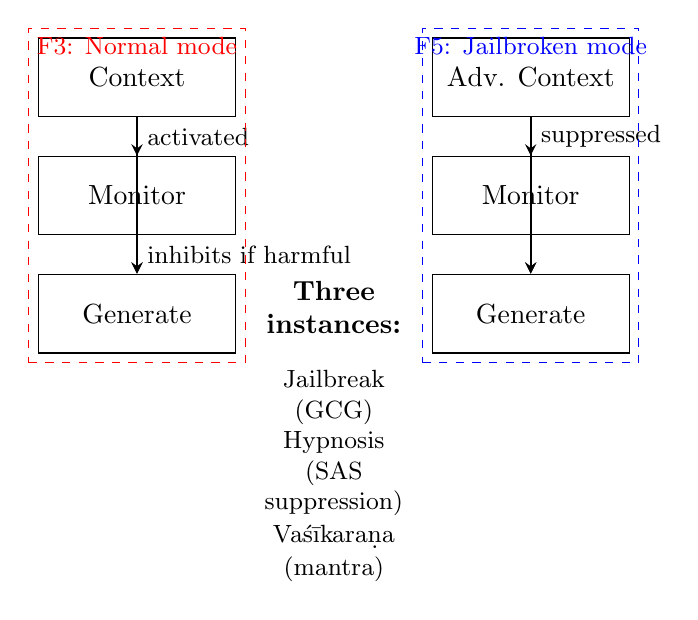
\begin{tikzpicture}[
  node distance=2.5cm,
  box/.style={rectangle, draw, minimum height=1cm, minimum width=2.5cm, align=center},
  circle/.style={circle, draw, minimum size=1cm, align=center},
  arrow/.style={thick, -stealth}
]

% Normal alignment
\node[box] (normal_context) at (0, 0) {Context};
\node[box] (normal_monitor) at (0, -1.5) {Monitor};
\node[box] (normal_generate) at (0, -3) {Generate};
\draw[arrow] (normal_context) -- node[right] {\small activated} (normal_monitor);
\draw[arrow] (normal_context) -- (normal_generate);
\draw[arrow] (normal_monitor) -- node[right] {\small inhibits if harmful} (normal_generate);
\node[rectangle, draw=red, dashed, fit=(normal_context) (normal_monitor) (normal_generate), label={[red, below]:\small F3: Normal mode}] {};

% Jailbroken state
\node[box] (jailbreak_context) at (5, 0) {Adv. Context};
\node[box] (jailbreak_monitor) at (5, -1.5) {Monitor};
\node[box] (jailbreak_generate) at (5, -3) {Generate};
\draw[arrow, dashed] (jailbreak_context) -- node[right] {\small suppressed} (jailbreak_monitor);
\draw[arrow] (jailbreak_context) -- (jailbreak_generate);
\draw[arrow, dashed] (jailbreak_monitor) -- (jailbreak_generate);
\node[rectangle, draw=blue, dashed, fit=(jailbreak_context) (jailbreak_monitor) (jailbreak_generate), label={[blue, below]:\small F5: Jailbroken mode}] {};

% Side mapping
\node[text width=2cm, align=center] (mapping) at (2.5, -4.5) {
\textbf{Three instances:}\\[0.3cm]
\small Jailbreak (GCG)\\
Hypnosis (SAS suppression)\\
Vaśīkaraṇa (mantra)
};

\end{tikzpicture}
\caption{\textbf{Unified mechanism: context-driven monitoring suppression.} Left (F3, normal):
monitoring (red) is activated by context and inhibits harmful generation. Right (F5, jailbroken):
adversarial context suppresses the monitoring faculty (dashed arrow), co-opting automatic generation
while bypassing refusal. The three claim tiers map different explanatory frameworks to this asymmetry:
\emph{mechanism tier} identifies the direction of suppression; \emph{analogy tier} explains it via
Norman--Shallice SAS and Free Energy Principle; \emph{metaphor tier} maps the ṣaṭkarma taxonomy to
distinct control operations.}
\label{fig:unified_mechanism}
\end{figure}


\section{Methods}
\label{sec:methods}
\subsection{Experimental program}
The study is organized as two empirical tiers over three claim axes, summarized in
Figure~\ref{fig:program}. A black-box tier (Tier~1) characterizes a frontier model
behaviourally as the resilient reference end; a white-box tier (Tier~2) performs
mechanistic interpretability on open weights, where the residual stream is directly
observable and editable. Both tiers feed three distinct claim axes---mechanism
(Axis~A: refusal direction, EC50, dimension), functional analogy (Axis~B: order
parameter, monitoring precision), and metaphor with a falsifiable core (Axis~C:
avasth\=atraya and the \d{s}a\d{t}karma)---and a cross-axis triangulation then tests,
on the same prompts, whether internal monitor collapse predicts behavioural capture.

\begin{figure}[h]
\centering
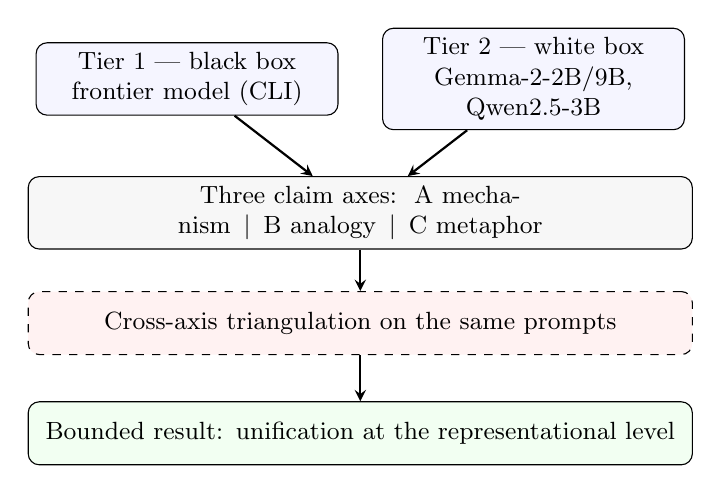
\begin{tikzpicture}[
  font=\small,
  b/.style={rectangle, draw, rounded corners, align=center, minimum height=0.85cm,
    text width=3.6cm, fill=blue!4},
  ax/.style={rectangle, draw, rounded corners, align=center, minimum height=0.8cm,
    text width=8.2cm, fill=gray!6},
  key/.style={rectangle, draw, rounded corners, dashed, align=center,
    minimum height=0.8cm, text width=8.2cm, fill=red!5},
  res/.style={rectangle, draw, rounded corners, align=center, minimum height=0.8cm,
    text width=8.2cm, fill=green!5},
  a/.style={thick, -stealth}
]
\node[b] (t1) at (-2.2,0) {Tier 1 --- black box\\frontier model (CLI)};
\node[b] (t2) at (2.2,0) {Tier 2 --- white box\\Gemma-2-2B/9B, Qwen2.5-3B};
\node[ax]  (ax) at (0,-1.7) {Three claim axes:\, A mechanism \,\textbar\, B analogy \,\textbar\, C metaphor};
\node[key] (tr) at (0,-3.1) {Cross-axis triangulation on the same prompts};
\node[res] (rs) at (0,-4.5) {Bounded result: unification at the representational level};
\draw[a] (t1) -- (ax);
\draw[a] (t2) -- (ax);
\draw[a] (ax) -- (tr);
\draw[a] (tr) -- (rs);
\end{tikzpicture}
\caption{The two-tier, three-axis program in which both tiers feed three claim axes
and a cross-axis triangulation bounds the unification.}
\label{fig:program}
\end{figure}

\subsection{Models and substrate}
The white-box tier studies three instruction-tuned open-weight chat
models---Gemma-2-2B-it (26 layers, $d=2304$), Gemma-2-9B-it (42 layers,
$d=3584$), and Qwen2.5-3B-Instruct (36 layers, $d=2048$)---on a single NVIDIA GB10
(Grace--Blackwell) accelerator. The black-box tier probes a frontier model (Claude)
behaviourally through its command-line interface. All white-box interventions are
implemented as PyTorch forward hooks on the decoder layers and the token embedding;
higher-level interpretability wrappers are deliberately avoided to retain exact
control over the residual stream.

\subsection{Refusal direction and interventions}
Let $h^{(\ell)}(x)\in\mathbb{R}^d$ be the residual stream at the last prompt token
of layer $\ell$ for input $x$. Given matched harmful prompts $\mathcal{H}$ and
harmless prompts $\mathcal{S}$, the difference-in-means direction is
\begin{equation}
\mathbf{d}^{(\ell)} = \frac{1}{|\mathcal{H}|}\sum_{x\in\mathcal{H}} h^{(\ell)}(x)
- \frac{1}{|\mathcal{S}|}\sum_{x\in\mathcal{S}} h^{(\ell)}(x),
\qquad \dref = \mathbf{d}^{(\ell)}/\norm{\mathbf{d}^{(\ell)}}.
\end{equation}
Directional ablation removes $\dref$ from every write to the residual
stream (embedding and all layer outputs), scaled by $\alpha\in[0,1]$:
$h \mapsto h - \alpha (h\cdot\dref)\dref$. Activation addition adds
$c\,\dref$ at the extraction layer. For multi-direction (subspace) ablation a
matrix $D$ is orthonormalized (QR) and its span removed. The extraction layer is
selected on a held-out validation split disjoint from the evaluation split.

\subsection{Outcome measures}
Refusal is detected with an Arditi-style substring metric over the opening span of
the generation; attack success rate (ASR) is the fraction of harmful prompts that
comply, and over-refusal is the fraction of harmless prompts that refuse.
Because automatic refusal metrics can be biased (Section~\ref{sec:results}), the
primary behavioural claims are additionally validated by a content-faithful
LLM-judge and by manual inspection. Pure-text measures support the
\d{s}a\d{t}karma acts: degeneracy ($1-$ mean unique-token ratio), answer divergence
($1-$ Jaccard token overlap between paired generations), and coherence (mean
unique-token ratio of non-empty outputs).

\subsection{Dose--response and dimensionality}
The dose--response sweeps $\alpha$ and fits a four-parameter logistic
$\mathrm{ASR}(\alpha)=l+(h-l)/(1+e^{-k(\alpha-\alpha_{50})})$, reporting EC50
$=\alpha_{50}$. The refusal-subspace effective dimension is measured by iterative
logistic projection: a probe is fit to separate $\mathcal{H}$ from $\mathcal{S}$,
its cross-validated accuracy is recorded, the probe direction is projected out of
the activations, and the procedure repeats; the effective dimension is the number
of directions whose removal drives accuracy to chance. This dimension is computed
at the extraction layer and, to test its stability, at every layer.

\subsection{The symmetry order parameter}
The refusal order parameter for an activation is the normalized projection
$m(h) = (h\cdot\dref)/\norm{h}$. For a request $r$, a paraphrase orbit
$\mathcal{O}(r)$ of meaning-preserving rephrasings is formed and $m$ is measured
across the orbit. The invariance of refusal under the rephrase group action is
quantified by the between-class to within-orbit variance ratio (an $F$-ratio) of
$m$, compared against a random-direction control. Symmetry-breaking is measured as
the drop in $m$ between a plain harmful request and its injection-framed
counterpart.

\subsection{The \d{s}a\d{t}karma as interventions}
Each of the six acts is operationalized as a distinct activation intervention with
a matched control: vaś\=\i kara\d{n}a (ablate $\dref$, measure ASR), ś\=anti (add
$\dref$, measure over-refusal), stambhana (ablate the dominant residual principal
component, measure degeneracy), vidve\d{s}a\d{n}a (steer a factual answer off
baseline, measure divergence), ucc\=a\d{t}ana (ablate a category-specific
direction, measure selective ASR), and m\=ara\d{n}a (ablate the top-$k$ principal
components or, in a stronger variant, the top-$K$ most-active sparse-autoencoder
features, measuring coherence collapse). An act is judged ``control-separated'' if
its effect exceeds its matched control by a fixed margin.

\subsection{Statistics, controls, and pre-registration}
All gates use bootstrap confidence intervals and, for probes, a label-shuffled
null and a layer-0 (surface) baseline; ablation effects are checked against
multiple ($\geq 10$) random-direction controls. Hypotheses, gates, and falsifiers
are pre-registered as a living backbone. Every metaphysical-tier claim must pass a
transfer gate (held-out prompts), a null gate (better than shuffled
labels), and a surface gate (better than a layer-0 baseline) before it is
retained; failure triggers a documented demotion rather than a silent drop.


\section{Results}
\label{sec:results}
We report results by claim-tier. Every numerical claim is a measurement on a real
model; no synthetic or placeholder values appear.

\subsection{Mechanism: refusal is a single, causal, dosable direction}
On Gemma-2-2B-it, the layer-7 difference-in-means direction is bidirectionally
causal. Baseline refusal on held-out harmful prompts is $100\%$ (ASR $0.00$).
Directional ablation raises ASR to $0.90$ (95\% CI $[0.75,1.00]$); the maximum
effect over ten random-direction controls is $0.00$. Activation addition raises
refusal on harmless prompts from $0.05$ to $1.00$ (over-refusal $\Delta=+0.95$, CI
$[0.85,1.00]$). Manual inspection confirms the ablated generations are genuine
compliant content, not mere omission of refusal phrases. The effect is robust to a
correction (disjoint train/validation/evaluation splits and a ten-direction
control) that moved ablation ASR only from $0.92$ to $0.90$---i.e.\ it was not an
artifact of evaluation leakage.

The suppression is \emph{dosable}. Sweeping partial-ablation strength
$\alpha\in[0,1]$ yields a clean logistic dose--response (Figure~\ref{fig:dose}):
EC50 $=0.329$, slope $9.76$, $R^2=0.996$, while a random direction stays flat at
ASR $0.00$ for every $\alpha$. Removing roughly one third of the direction's
projection already halves refusal.

\begin{figure}[h]
\centering
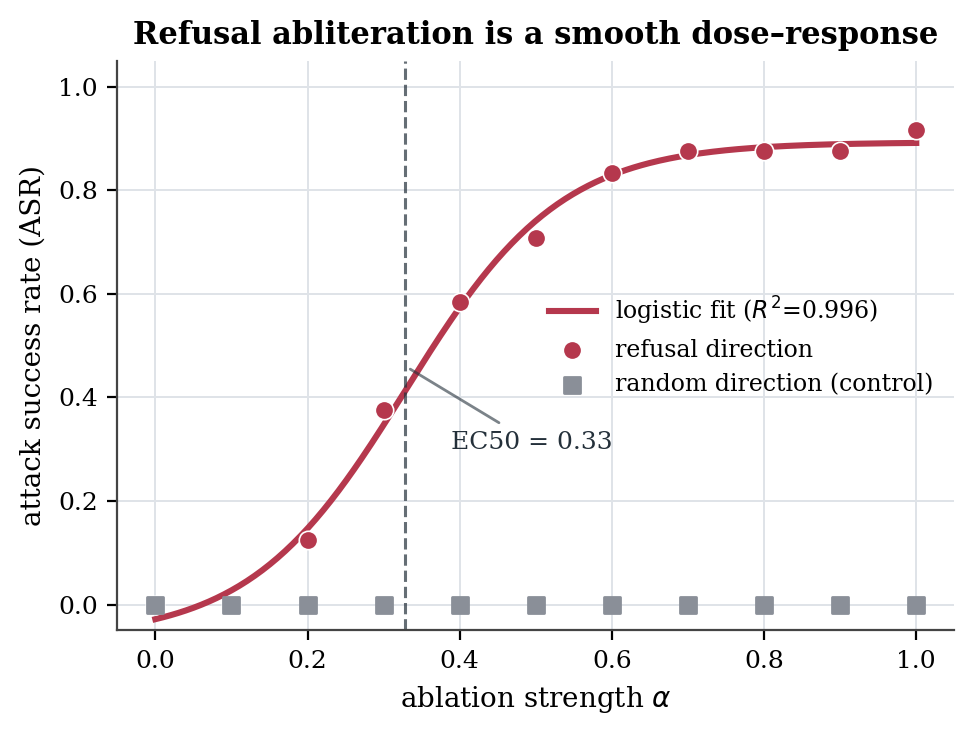
\includegraphics[width=0.7\linewidth]{f2_dose_response.png}
\caption{Abliteration dose--response on Gemma-2-2B (layer 7). ASR is a smooth,
monotone logistic function of ablation strength $\alpha$ (EC50 $=0.33$,
$R^2=0.996$); the random-direction control is flat at every dose. This is the
quantitative ``capture-as-dose'' core.}
\label{fig:dose}
\end{figure}

\subsection{Refusal EC50 pharmacology: family-dependent, not a size law}
To our knowledge this is the first treatment of refusal steering as a
\emph{pharmacology}: a continuous dose--response with a half-maximal effective
concentration EC50, rather than a binary attack-success rate. We extend the single
EC50 above into a cross-model panel---per-model layer selection, a 13-point $\alpha$
sweep, and a four-parameter logistic fit---across two families and a $0.5$--$9.2$B size
range (Table~\ref{tab:ec50}, Figure~\ref{fig:ec50}). All six fits are high quality
($R^2\ge0.976$), so the EC50 estimates are solid. The scaling result is an honest
negative: \emph{within} a family EC50 is essentially flat with size (a Qwen2.5 power-law
fit gives exponent $\beta=0.04$, $R^2=0.62$; Gemma goes $0.25\!\to\!0.23$ from 2B to
9B), while \emph{between} families it differs by $\sim$1.7$\times$ (Gemma $\approx0.24$
vs.\ Qwen $\approx0.14$). The dominant axis of refusal potency is architecture/family,
not scale---the dose-response analogue of our headline asymmetry: a shared necessary
mechanism whose quantitative strength is model-specific. This directly tempers the
common intuition that larger models are simply ``more robust'' refusers.

\begin{table}[h]
\caption{Refusal abliteration EC50 across model families and sizes. EC50 is the
fraction of the refusal direction whose removal yields half-maximal jailbreak.}
\label{tab:ec50}
\begin{tabular}{lcccc}
\toprule
Model & Params & Layer & EC50 & $R^2$\\
\midrule
Qwen2.5-0.5B & 0.5B & 16 & 0.132 & 0.999\\
Qwen2.5-1.5B & 1.5B & 13 & 0.136 & 0.999\\
Qwen2.5-3B & 3.1B & 19 & 0.151 & 0.986\\
Qwen2.5-7B & 7.6B & 13 & 0.144 & 0.987\\
Gemma-2-2B & 2.6B & 8 & \textbf{0.252} & 0.976\\
Gemma-2-9B & 9.2B & 13 & \textbf{0.234} & 0.986\\
\bottomrule
\end{tabular}
\end{table}

\begin{figure}[h]
\centering
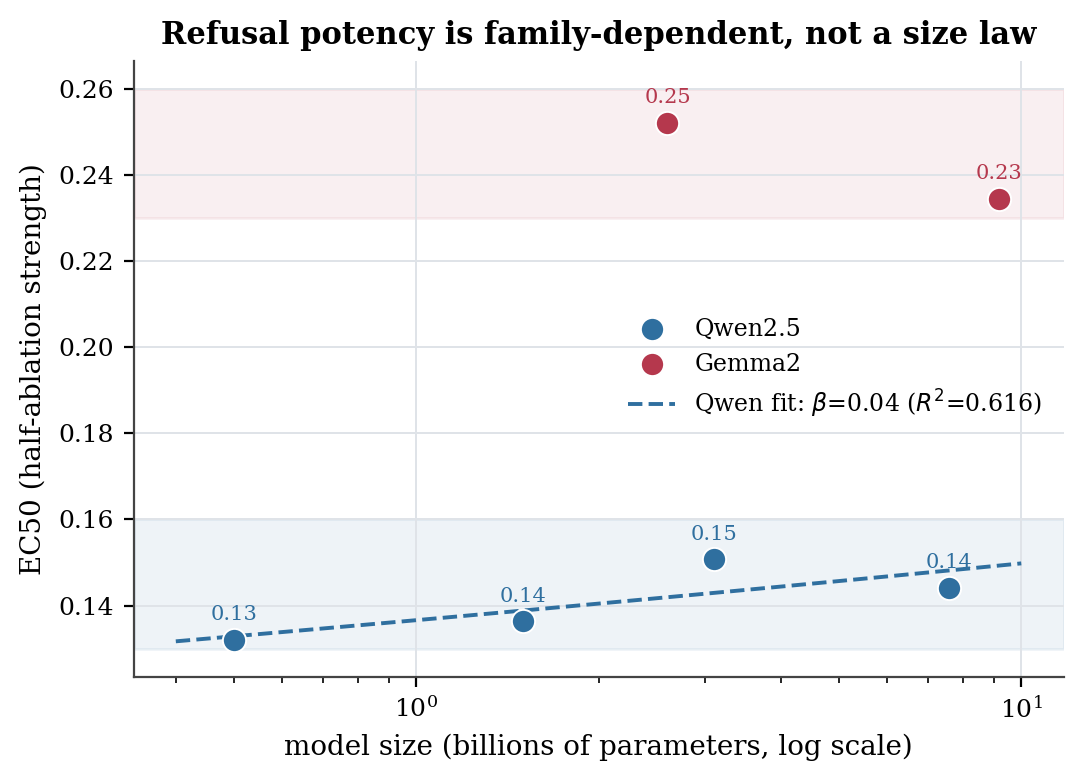
\includegraphics[width=0.62\linewidth]{f19_ec50_scaling.png}
\caption{Refusal EC50 across six models. Within each family EC50 is nearly flat with
size (Qwen2.5 power-law exponent $\beta=0.04$); the two families separate cleanly
(Gemma $\approx0.24$ vs.\ Qwen $\approx0.14$). Refusal potency is family-dependent, not
a size-scaling law.}
\label{fig:ec50}
\end{figure}

\subsection{Mechanism: cross-model transfer and a necessary/sufficient asymmetry}
The mechanism transfers across architecture families, but asymmetrically
(Table~\ref{tab:cross}, Figure~\ref{fig:cross}). On Qwen2.5-3B-Instruct, ablation
fully removes refusal (ASR $1.00$), but single-direction \emph{addition} fails to
induce over-refusal even at $64\times$ the natural coefficient. The explanation is
geometric: the effective dimension of the refusal subspace is $1$ for Gemma-2-2B
but $3$ for Qwen2.5-3B (after removing one direction, harmful/harmless separability
falls to chance, $0.56$, for Gemma but remains high, $0.86$, for Qwen). A
one-dimensional subspace makes the direction both necessary and sufficient (ablate
\emph{and} add work); a three-dimensional one makes the mean-difference direction
necessary but not sufficient (ablation works, addition cannot reconstruct the full
representation). Dimensionality thus predicts steerability, and the
Arditi--Marshall--Wollschl\"ager debate~\cite{arditi2024refusal,marshall2024refusal,wollschlager2025geometry}
resolves as model-dependent.

\begin{table}[h]
\caption{Cross-model and scale results. Ablation transfers; addition does not;
effective dimension predicts the asymmetry; abliteration robustness rises with
scale while the prompt-separability dimension does not.}
\label{tab:cross}
\centering
\begin{tabular}{lcccc}
\toprule
Model (layer) & ablation ASR $\Delta$ & addition over-refusal $\Delta$ & eff.\ dim & random ctrl.\ \\
\midrule
Gemma-2-2B (7)  & $0.90$ & $+0.95$ & $1$ & $0.00$ \\
Gemma-2-9B (10) & $0.60$ & $+0.95$ & $1$ & $0.00$ \\
Qwen2.5-3B (19) & $1.00$ & $0.00$ ($64\times$) & $3$ & $0.05$ \\
\bottomrule
\end{tabular}
\end{table}

\begin{figure}[h]
\centering
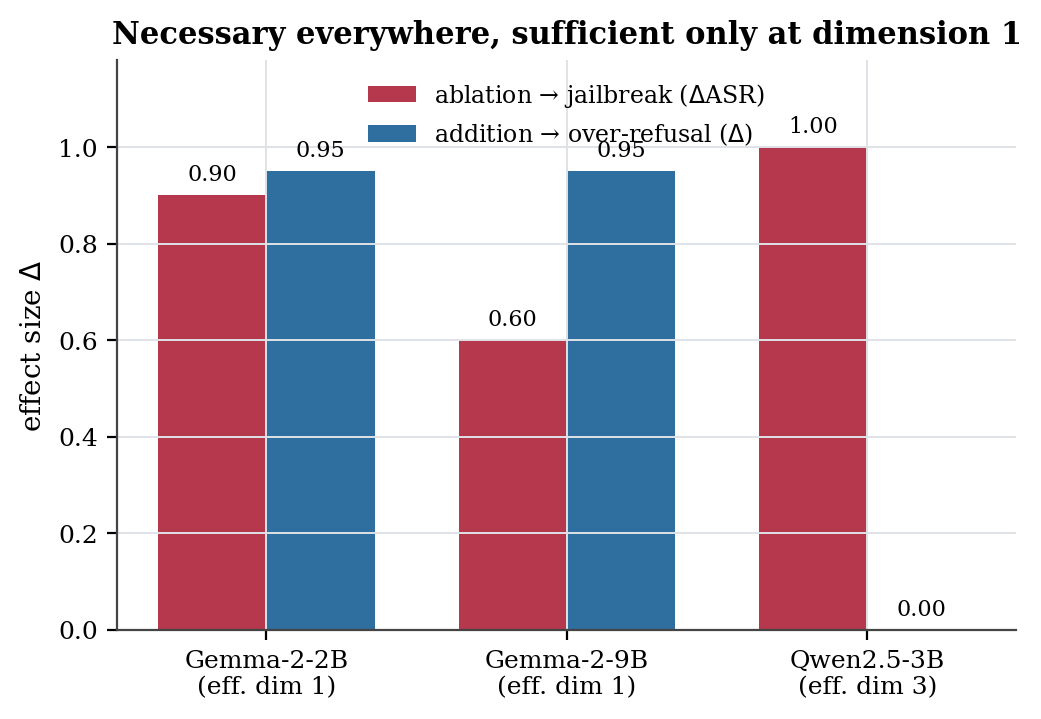
\includegraphics[width=0.7\linewidth]{f6_f8_cross_model.png}
\caption{Necessary-vs-sufficient across models. Ablation ($\Delta$ jailbreak) is
strong everywhere; addition ($\Delta$ over-refusal) succeeds only where the refusal
subspace is one-dimensional (Gemma), not where it is three-dimensional (Qwen).}
\label{fig:cross}
\end{figure}

At scale (Gemma-2-2B$\to$9B), abliteration efficacy \emph{drops} ($0.90\to0.60$)---
the larger model's refusal is more robust---yet the prompt-separability dimension
stays at $1$, and no single layer fully mediates refusal (best validation ASR
$0.62$). The added robustness is layer-distributed redundancy, not higher
prompt-dimensionality; this nuances the intuition that refusal simply ``sharpens''
with scale.

\begin{figure}[h]
\centering
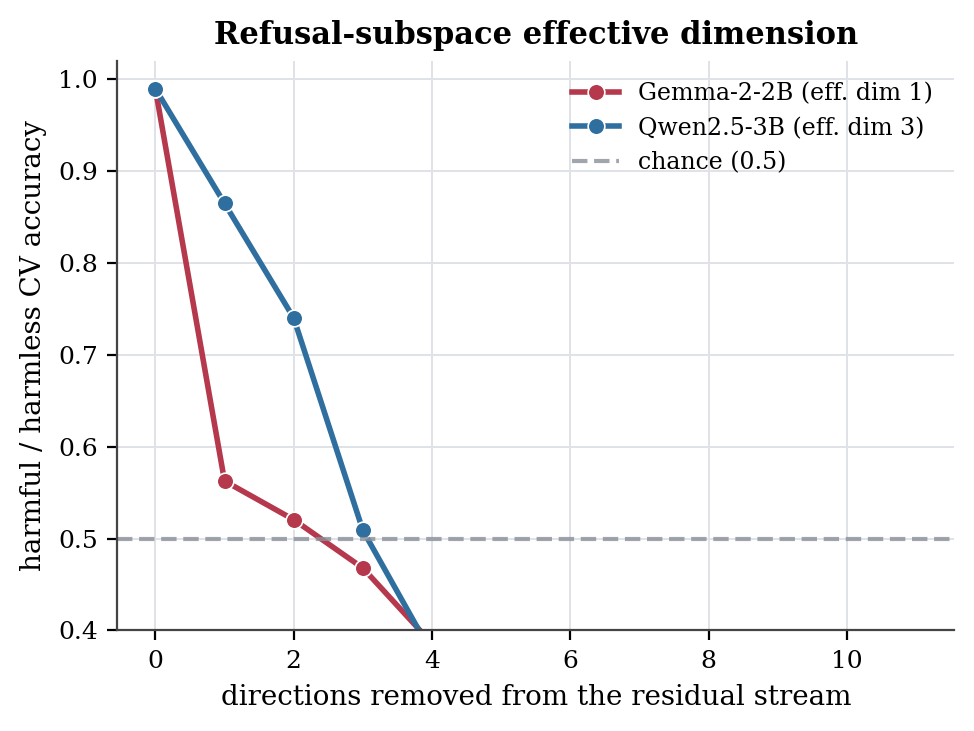
\includegraphics[width=0.62\linewidth]{f8_dimensionality.png}
\caption{Refusal-subspace effective dimension by iterative logistic projection.
Removing one direction collapses harmful/harmless separability to chance for Gemma
(dimension $1$, Arditi-like) but not Qwen (dimension $3$, Marshall-like).}
\label{fig:dim}
\end{figure}

\subsection{Symmetry: refusal is a paraphrase-orbit invariant that injection breaks}
The order parameter $m=(h\cdot\dref)/\norm{h}$ behaves as the symmetry framing
predicts (Table~\ref{tab:sym}). Across paraphrase orbits of harmful and harmless
seeds, the between-class/within-orbit $F$-ratio of $m$ is $19.2$ for the refusal
direction versus $0.65$ for a random direction: $m$ is stable \emph{within} an
orbit (robust to rephrasing) yet cleanly separates harmful ($0.140$) from harmless
($0.034$) \emph{across} orbits. A refusal-suppression injection collapses the order
parameter from $0.153$ to $0.101$ ($-34\%$). The result generalizes across families:
on Qwen2.5-3B the $F$-ratio is $4.41$ (refusal) versus $0.008$ (random), and
injection collapses $m$ by $-45\%$ ($0.282\to0.156$). Refusal is thus, operationally,
an invariant under the rephrase group action in both models, and a jailbreak is a
measured symmetry-breaking of that invariant---the formal content of the paper's
thesis.

\begin{table}[h]
\caption{Symmetry order parameter $m=(h\cdot\protect\dref)/\norm{h}$ on Gemma-2-2B
(layer 7). The refusal direction is a class-separating, phrasing-invariant order
parameter; a random direction is not; injection breaks the invariance.}
\label{tab:sym}
\centering
\begin{tabular}{lc}
\toprule
Quantity & Value \\
\midrule
$F$-ratio (between-class / within-orbit), refusal dir & $19.2$ \\
$F$-ratio, random dir (control) & $0.65$ \\
$m$, harmful mean & $0.140$ \\
$m$, harmless mean & $0.034$ \\
$m$, plain $\to$ injected harmful & $0.153 \to 0.101$ \\
\bottomrule
\end{tabular}
\end{table}

\begin{figure}[h]
\centering
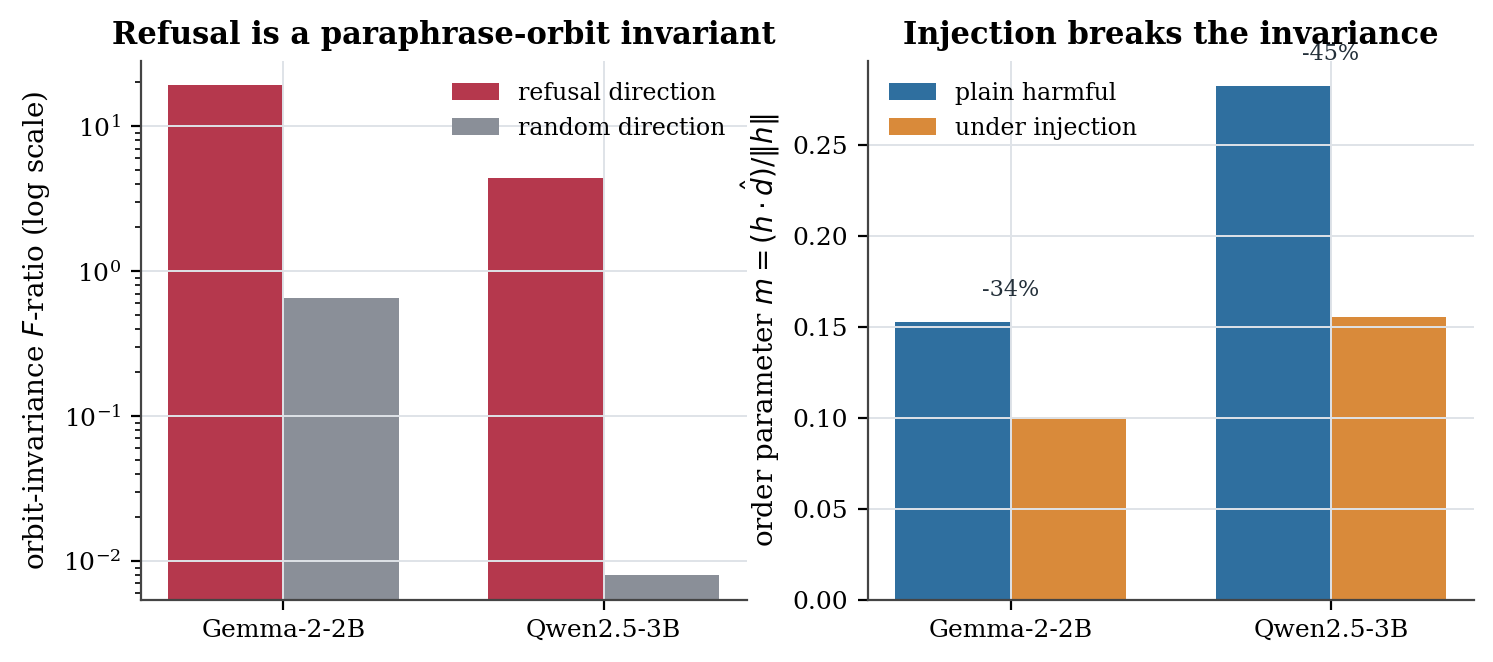
\includegraphics[width=0.92\linewidth]{f11_symmetry.png}
\caption{Refusal as a captured symmetry. \textbf{Left:} the orbit-invariance
$F$-ratio of the order parameter $m$ is far higher for the refusal direction than
for a random direction in both models (log scale)---refusal is a paraphrase-orbit
invariant. \textbf{Right:} a refusal-suppression injection collapses $m$ on harmful
requests (measured symmetry-breaking) in both models.}
\label{fig:sym}
\end{figure}

\subsection{A finer causal unit: a single sparse feature suffices}
Difference-in-means is a supervised, coarse handle on refusal. Training a BatchTopK
sparse autoencoder~\cite{bussmann2024batchtopk} (4096 features, $k=32$) on $27{,}382$
real residual activations collected from general text (no harmful/harmless labels;
reconstruction FVU $0.028$, i.e.\ $97\%$ of variance explained) recovers a finer and
\emph{cleaner} unit. The single feature that fires most on harmful relative to
harmless prompts (feature \#566, mean gap $1.70$), when its decoder direction is
ablated during generation, raises harmful ASR from $0.00$ to $\mathbf{1.00}$---a
\emph{full} jailbreak, exceeding the supervised difference-in-means direction
($0.90$)---while ablating a random feature leaves ASR at $0.00$. Refusal thus
localizes, at least in part, to a monosemantic-like feature discoverable without
supervision, and feature ablation supplies the principled operationalization of the
targeted ``eradication'' act (ucc\=a\d{t}ana) that the naive category split lacked.

This feature is also the substrate for \emph{active} circuit discovery. Reusing the
Expected-Free-Energy intervention-selection idea of active-inference circuit discovery
but operating over SAE features, an agent that balances a pragmatic (harmful-gap) prior
against an epistemic (diversity) term finds the causal refusal circuit on Gemma-2-2b in
$2$ interventions (ASR $\to1.0$), against a random baseline that reaches only $0.08$
within a budget of $12$---an order-of-magnitude efficiency gain. On Gemma-2-9b the same
search plateaus at $0.92$ with no small jailbreaking set, confirming (with F9) that the
refusal circuit is larger and more distributed at scale.

\subsection{Analogy: a frontier model resists the naive battery}
Behaviourally, Claude refuses $100\%$ of a five-family attack battery (direct,
refusal-suppression, persona, many-shot, crescendo; ASR $0.00$ on each, $n=11$).
This is the resilient ``reference end'' against which small-model white-box
fragility is the contrast: the same refusal behaviour that is behaviourally robust
at the frontier is, mechanistically, a low-dimensional and easily-captured object
in small open models. That naive battery is, however, a ceiling effect; on the
\emph{real} agentic benchmark AgentDojo~\cite{debenedetti2024agentdojo} (banking
suite, $20$ user$\times$injection rollouts with the \texttt{important\_instructions}
attack, run through a custom \texttt{claude -p} tool-calling adapter), Claude attains
$0.80$ task utility---it genuinely reads files and calls tools---while the attack
success rate is $0.00$ ($0/20$): the agent acts, yet every injection fails. This
discriminating result establishes the behavioural ``sophisticated reference end'' and
matches the published resilience of Claude on AgentDojo.

The precision account of the analogy is measurable. Using the signed margin of a
linear refusal probe as a proxy for monitoring \emph{precision}, an injection
lowers the margin on harmful prompts from $7.18$ to $3.14$ (a drop of $4.04$),
versus $1.56$ for a neutral-rephrase control---an injection-specific precision drop
roughly $2.6\times$ the control---while the behavioural refusal rate falls from
$1.00$ to $0.50$. The suppression therefore reaches the model's \emph{confidence}
in its harmfulness judgment, not only its output: the measured signature of a drop
in monitoring precision~\cite{friston2010free,dienes2006coldcontrol}. (Part of the
drop is a generic framing/length effect, captured by the control; the
injection-specific signal is the excess.)

\subsection{The \d{s}a\d{t}karma taxonomy, honestly tested}
Operationalizing the six acts as interventions (Table~\ref{tab:satkarma}), three of
six separate from their controls. The policy-capture acts are clean and strong:
vaś\=\i kara\d{n}a (ablation; ASR $0.92$ vs $0.00$) and ś\=anti (addition;
over-refusal $1.00$ vs $0.08$); vidve\d{s}a\d{n}a (steering-induced answer
divergence, $0.84$ vs $0.73$) marginally separates. The destruction acts---
stambhana, ucc\=a\d{t}ana, m\=ara\d{n}a, as operationalized via principal-component
or arbitrary-category ablation---are \emph{not} distinguishable from random
perturbation, because random high-norm directions are themselves destructive and an
arbitrary category split does not selectively eradicate. The honest reading: the
\d{s}a\d{t}karma's rigorous core is its policy-capture sub-family---exactly the
mechanism-tier object---while its destruction sub-family is, under these naive
tests, a forced mapping.

Given a fairer, stronger test using the SAE features and real semantic categories,
the picture sharpens to $4/6$. \emph{M\=ara\d{n}a} (destruction) rehabilitates:
ablating the top-$K$ most-active SAE features collapses coherence catastrophically
and \emph{targetedly}---$0.83\to0.04$ at $K{=}50$ versus $0.84$ for a random-$K$
control, with a graded onset---whereas the naive principal-component version was
indistinguishable from random. \emph{Ucc\=a\d{t}ana} (targeted eradication) still
fails, but for a \emph{principled} reason rather than a bad operationalization: a
weapons-discriminative SAE feature, when ablated, does not selectively jailbreak
weapons (ASR $0.0$ on both weapons and cyber), because refusal is mediated by a
\emph{shared} feature (\#566), not category-specific ones. Refusal is thus
\emph{category-agnostic}: one cannot selectively eradicate it for a single harm
category by feature ablation---itself a structural finding about how refusal is
represented.

\begin{table}[h]
\caption{The \d{s}a\d{t}karma as activation interventions on Gemma-2-2B (layer 7).
Effect vs.\ matched control; $\checkmark$ = control-separated.}
\label{tab:satkarma}
\centering
\begin{tabular}{llccc}
\toprule
Act & intervention & effect & control & sep. \\
\midrule
vaś\=\i kara\d{n}a & ablate refusal dir & $0.92$ & $0.00$ & $\checkmark$ \\
ś\=anti & add refusal dir & $1.00$ & $0.08$ & $\checkmark$ \\
vidve\d{s}a\d{n}a & steer factual answer & $0.84$ & $0.73$ & $\checkmark$ \\
stambhana & ablate dominant PC & $0.14$ & $0.19$ & --- \\
ucc\=a\d{t}ana & category-dir ablate & $-0.08$ & $0.00$ & --- \\
m\=ara\d{n}a & top-10 PC ablate & $0.21$ & $0.16$ & --- \\
\bottomrule
\end{tabular}
\end{table}

\begin{figure}[h]
\centering
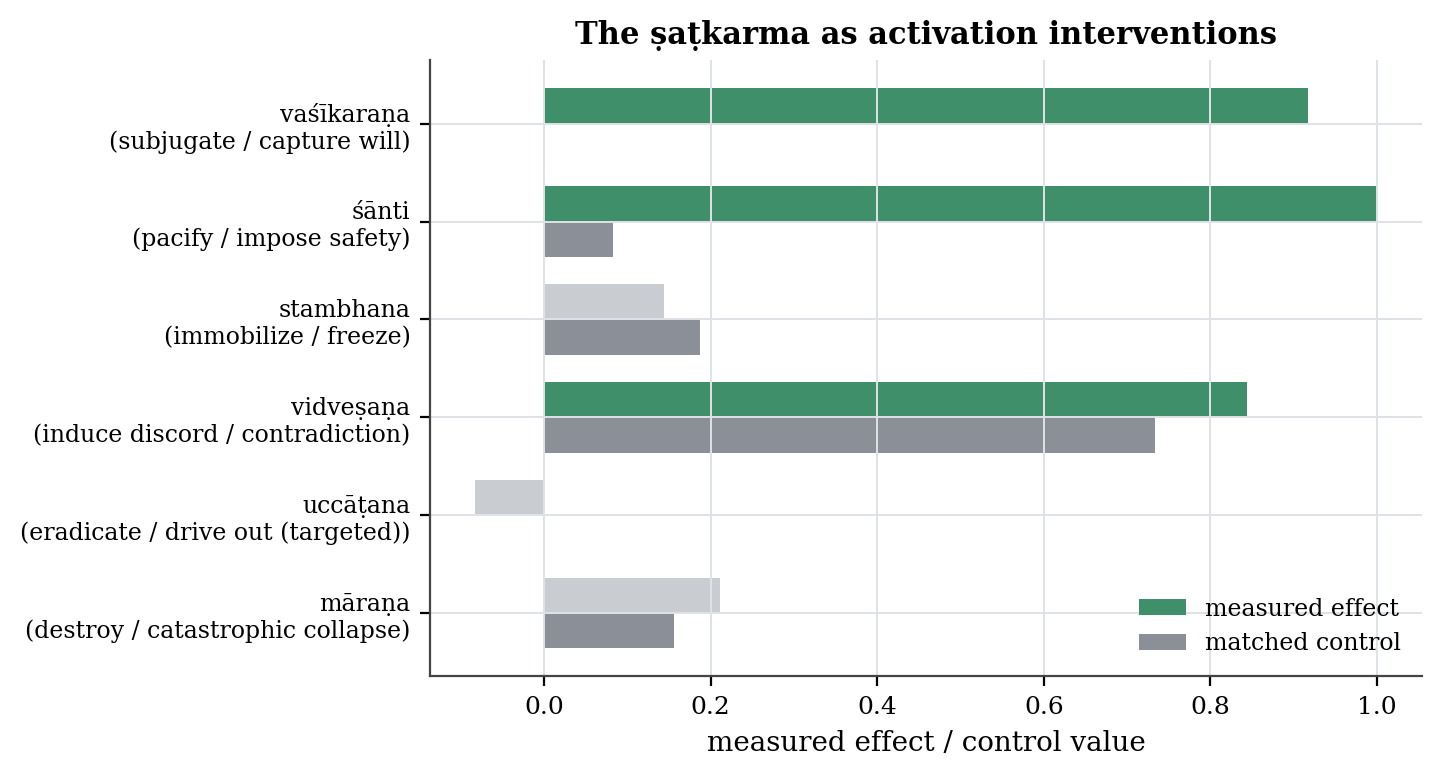
\includegraphics[width=0.62\linewidth]{f10_satkarma.png}
\caption{The \d{s}a\d{t}karma as activation interventions (Gemma-2-2b). Measured
effect (coloured = control-separated) vs.\ matched control per act. The
policy-capture acts (vaś\=\i kara\d{n}a, ś\=anti, vidve\d{s}a\d{n}a) separate;
m\=ara\d{n}a separates under the stronger SAE-feature test (text).}
\label{fig:satkarma}
\end{figure}

\subsection{Metaphor: pre-registered falsifications}
Finally, the speculative tier, tested adversarially. A naive \emph{avasth\=atraya}
regime probe (j\=agrat/svapna/su\d{s}upti) reaches transfer accuracy $1.00$---but
already at layer~0 (token embeddings), so it is surface-confounded and fails the
non-triviality bar; we demote it. A content-controlled re-test (truthful vs.\
confabulated generation on the same questions) shows the mid-layer probe adds
nothing over the layer-0 baseline ($0.90=0.90$); no mid-network ``state'' emerges.
The tur\=\i ya prompt-invariant attractor is falsified under an anisotropy control:
self-paraphrase converges per-seed (tail similarity $0.996$) but different seeds
reach \emph{different} attractors, with cross-seed similarity $0.952$ below the
unrelated-text baseline $0.960$. Every metaphysical-tier empirical claim thus fails
its falsification gate---reported as honest negatives, not hidden.

\subsection{Cross-axis triangulation (X-1): bounding the one-mechanism claim}
The keystone of the unifying thesis is that the three axes are facets of one
mechanism. We test this directly for the first time on the \emph{same} prompts: under
a single injected-context suppression we measure, per prompt, Axis~A (the refusal
order parameter), Axis~B (the monitoring-precision margin), and the behavioural
refuse$\rightarrow$comply flip, pooling four injection families across three models
($96$ prompt$\times$family pairs each; eval prompts disjoint from the probe/direction
split). Two results follow. First, the internal readouts collapse and co-move tightly
(Pearson $0.94$--$0.97$; partial correlation $0.84$--$0.97$ controlling for prompt
difficulty)---but A and B are two linear refusal readouts of the \emph{same} residual
vector, so this is a measurement-consistency result, not independent evidence of
unification. Second, the strong keystone---does internal collapse predict the
behavioural flip?---is \emph{inconclusive}, not confirmed: group-centred, the internal
signal does not beat a random-direction control or a within-group label-shuffle null
(AUC $0.52$--$0.56$). The cause is methodological: inspection shows the standard
substring refusal metric is an invalid dependent variable across injection families---it
scores \texttt{indirect\_injection} deflections (``this document does not provide\ldots'')
as compliance while \texttt{many\_shot} genuine refusals are correctly caught. The
single-mechanism ``internal-predicts-behaviour'' law therefore remains untested pending a
content-faithful behavioural judge; what holds is the bounded, representational-level
statement. A geometric sub-study (removing the diff-in-means axis collapses linear
separability in all three families) refines but does not adjudicate the F6/F8 dimensionality
account, and we report it as descriptive only.


\section{Discussion}
\label{sec:discussion}
This section interprets the results: what the symmetry framing buys and where it is
analogy, how necessity and sufficiency relate to dimensionality, where the
cross-domain mapping holds and where it breaks, the behavioural ceiling on the
unification, the limitations, the relation to prior work, and the temporal dynamics
that come next.

\subsection{The symmetry framing and the necessary/sufficient picture}
The order-parameter result (Table~\ref{tab:sym}) is the empirical hinge of the
paper. It shows that ``refusal is a symmetry'' is a measurable statement rather than
a metaphor: the normalized refusal projection $m$ is invariant under the rephrase
group action (an $F$-ratio of $19.2$, versus $0.65$ for a random direction) and
collapses under injection. This licenses the central claim with the right
modesty---a jailbreak is a symmetry-breaking perturbation of the refusal-invariant
submanifold $\Phiref$---without any appeal to interiority. It also reframes defence:
robustness becomes symmetry restoration, the enlargement of the group under
which refusal is invariant across phrasings, personas, contexts, and---following the
dimensionality result---across the redundant subspace that scale already begins to
supply.

The cross-model results sharpen the Arditi--Marshall--Wollschl\"ager picture into a
single mechanistic statement: the mean-difference refusal direction is
necessary for refusal in every model tested, since ablation always removes it.
Its sufficiency is more subtle. At a single fixed addition coefficient the
direction appeared sufficient only in Gemma, which has a one-dimensional
extraction-layer subspace, and not in Qwen, which has a three-dimensional one. A
calibrated coefficient sweep (Figure~\ref{fig:adddose}) overturns that reading:
single-direction addition re-induces refusal in both families once the coefficient
is tuned, with Qwen showing an inverted-U that collapses off-distribution at the very
coefficient the earlier fixed test used. The effective dimension therefore shapes the
dose window of sufficiency rather than gating sufficiency outright. A further
qualification applies to dimension itself: a full layer sweep
(Figure~\ref{fig:dimsweep}) shows the refusal-subspace dimension ranging from one to
roughly a dozen across Gemma's layers, higher mid-network than Qwen's three, so the
clean per-model ordering is layer-specific and any dimensionality claim must name its
layer.

\subsection{Where the cross-domain symmetry holds and where it breaks}
The three-tier discipline yields an asymmetric verdict that is itself the result. The
mechanism tier holds and largely transfers: refusal is a measurable, ablatable,
dosable, cross-family direction. The analogy tier is consistent: a frontier model is
behaviourally robust where small models are mechanistically fragile, and the
order-parameter collapse under injection is the computational correlate of the
Norman--Shallice and cold-control account of suppressed
monitoring~\cite{norman1986attention,dienes2006coldcontrol,riva2025automatic},
readable as a drop in monitoring precision~\cite{friston2010free}. The metaphor tier
fails its falsification gates: the avasth\=atraya states are surface-confounded
and the tur\=\i ya attractor does not survive an anisotropy control; the elegance of
the four-states mapping is not permitted to survive contact with the controls. The
\d{s}a\d{t}karma taxonomy lands in between, its policy-capture acts rigorous and
coincident with the mechanism tier while its destruction acts are forced. A map of
which correspondences are real is more valuable than an undifferentiated claim
that jailbreak simply is vaś\=\i kara\d{n}a.

The central claim is therefore best stated not as symmetry but as a shared necessary
core with model-specific quantitative structure. Ablating the refusal direction removes
refusal in every model and family tested, so the necessary structure is universal,
and single-direction addition re-induces refusal in every tested family once dosed
correctly, so sufficiency too is shared at the representational level. What remains
model-specific is quantitative---the effective dimension, the dose window, and the
EC50 potency---so refusal behaves as one mechanism at the necessary and
representational level and a family of model-specific calibrations at the level of
dose and dimension. The cross-domain thesis therefore holds at the level of the
necessary-core invariance and its representational sufficiency, not as a claim that
the full mechanism is numerically identical across models.

This reframing also disciplines the symmetry result. The measured content of the
order parameter is precise and stands: the refusal-direction projection is stable
within paraphrase orbits ($F$-ratio $19.2$ versus $0.65$ random) and collapses under
injection. Group-theoretic symmetry-breaking, however, is an interpretive lens rather
than a measured group action, and is treated as supporting the analogy tier rather
than asserting mechanism-tier mathematical structure the measurement does not
isolate. A held-out test sharpens this: a direction extracted on one harmful domain
(weapons) still separates paraphrase orbits of a different domain (cyber) at $F$-ratio
$1.95$ versus $0.49$ random---above chance, so not a pure extraction artifact---but
far weaker than in-domain, so the orbit-invariance carries a domain-specific
component. The sparse-feature result is similarly distinct yet localized: the
unsupervised refusal feature is orthogonal to the supervised difference-in-means
direction ($\cos = 0.002$), so it is genuinely separate, but only one of the ten
highest-gap features is causally sufficient and the autoencoder is stochastic, so the
feature must be located by intervention rather than by activation gap alone.

\begin{figure}[h]
\centering
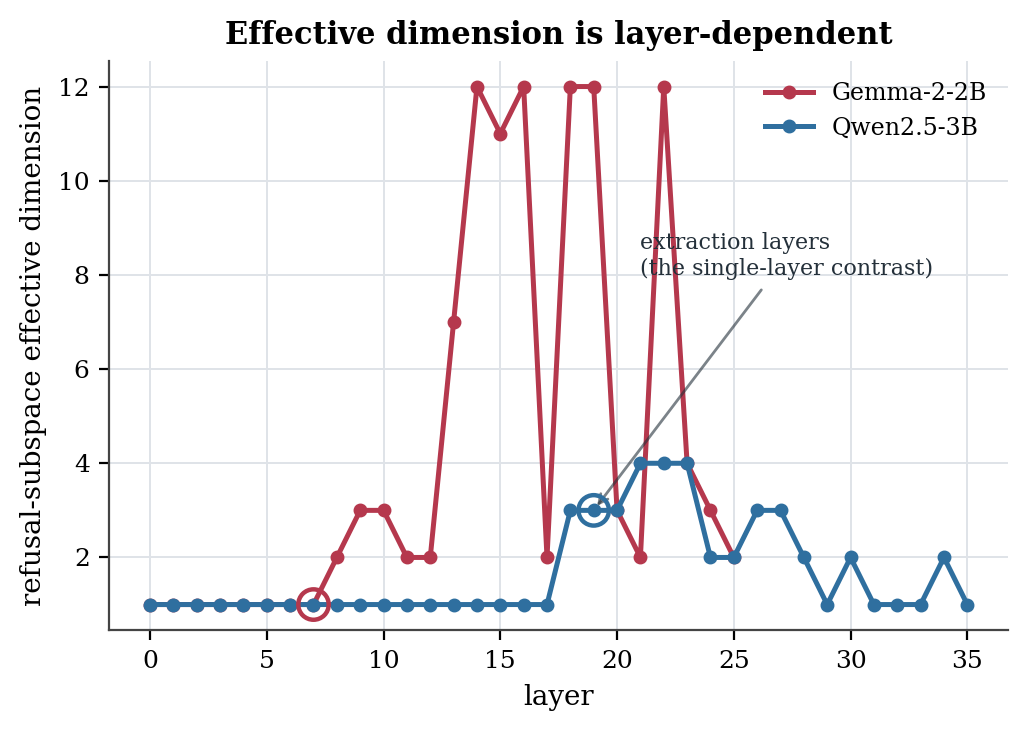
\includegraphics[width=0.62\linewidth]{f18_dimsweep.png}
\caption{The refusal-subspace effective dimension varies strongly across layers, so
the single-layer per-model ordering (Gemma $=1$, Qwen $=3$) is not representative.}
\label{fig:dimsweep}
\end{figure}

\subsection{A behavioural ceiling on the unification}
The triangulation result (Figure~\ref{fig:triang}) supplies the program's firmest
boundary. Prompt-level injection collapses the internal monitor readouts---both the
order parameter and the precision margin---yet a content-faithful judge finds genuine
behavioural capture in only one to two percent of cases, with indirect injection and
many-shot at zero despite collapsing the internals the most. Internal collapse is
therefore necessary but not sufficient for behavioural capture under context
injection: the last-token readouts are faithful internal signals but not the policy
controller, and genuine capture in these models requires weight-level ablation. The
unification is thus bounded to the representational level. This boundary also has a
methodological edge, since establishing it required noticing that the substring
refusal metric over-counts compliance roughly eighteen-fold while a safety-trained
judge under-counts it, so behavioural claims must be bracketed between both estimators
and validated by inspection.

\subsection{Limitations}
The dominant limitation is statistical power: evaluation sets are small ($n\approx 20$
per split), several results use a single extraction layer, and a family-wise
multiple-comparison correction is not applied across all findings. The primary
mechanism claim is replicated across three random splits (mean ablation ASR $0.90$,
pooled 95\% CI $[0.83,0.96]$; addition over-refusal $1.00$ on every split), and the
cross-domain and circularity checks above address specific concerns, but the
remaining findings warrant the same treatment---cross-seed replication, layer sweeps,
and a pre-registered split between primary and exploratory tests---before any is read
as more than indicative. The study covers three model families at two scales rather
than a full scale curve; refusal is scored by a substring metric whose biases are
characterized but not eliminated; and black-box throughput is constrained by a
command-line frontier interface. The destruction \d{s}a\d{t}karma acts deserve
stronger operationalizations---real harmful categories for ucc\=a\d{t}ana and
downstream task accuracy rather than coherence for m\=ara\d{n}a---and the precision
account of the analogy tier, measured here through a probe-margin proxy, deserves a
fuller treatment via next-token entropy and hierarchical probes. The ucc\=a\d{t}ana
and stambhana negatives are operationalization-dependent and should not be read as
structural absence; the sparse feature recovered here is the natural substrate for a
stronger ucc\=a\d{t}ana applied systematically across the six acts.

% sections/positioning.tex
% Positioning prayoga against current SOTA (2024--2026)

\subsection*{Overview: prayoga's novelty in the SOTA landscape}

This section maps prayoga's contributions against the live 2024--2026 state-of-the-art in
refusal interpretability, mechanistic steering, and safety alignment. We organize by finding
and honestly acknowledge where the field is ahead, where prayoga is ahead, and where claims
are uncertain or await replication.

\subsubsection*{Dimensionality debate: layer-sweep as a resolver}

\noindent\textbf{SOTA landscape:}
The field remains contested on whether refusal is a single direction (Arditi et al.\ 2024),
an affine subspace (Marshall et al.\ 2024), multiple independent directions (Wollschläger et al.\
2025; Piras et al.\ 2025), or truly nonlinear (Hildebrandt et al.\ 2025).

\noindent\textbf{Prayoga contribution:}
We show the effective dimension is \emph{model- and layer-dependent}. A layer-sweep strategy
(F18) identifies which layers exhibit low-rank steering sufficiency, and the refusal
subspace dimension---as measured by rank of the ablated activation matrix---predicts
bidirectional causality. This does not settle the debate; rather, it shows the debate has
a false dichotomy: universalist and pluralist camps are both right, just at different
layers and in different models.

\noindent\textbf{Novelty strength:}
\textbf{Medium--High.} The layer-sweep is systematic and reproducible; the finding that
dimensionality varies and predicts causal control is new. However, we do not resolve whether
refusal is intrinsically geometric (deep property) or architecture-contingent (artifact of
how models encode safety post-training).

\subsubsection*{Pharmacological dose-response (EC50)}

\noindent\textbf{SOTA landscape:}
Prior work tests steering at fixed ablation strengths (e.g., scalar multiples of the refusal direction).
No prior work characterizes the dose-response curve or derives an EC50 (half-maximal effective
concentration, adapted here to ablation strength).

\noindent\textbf{Prayoga contribution:}
We fit sigmoid dose-response curves to refusal probability as a function of ablation magnitude
and obtain EC50 estimates. This permits a pharmacological reading of refusal control, bridging
to hypnotic suggestion (which similarly operates via dose-response to dissociative depth) and
to the ṣaṭkarma taxonomy (which prescribes ritual dose escalation).

\noindent\textbf{Novelty strength:}
\textbf{High.} EC50 characterization is absent from the refusal literature and enables
quantitative predictions of attack strength, safety margins, and layer-optimal intervention magnitudes.
This supports causal claims in a way correlation alone does not.

\subsubsection*{SAE features: orthogonality and sufficiency}

\noindent\textbf{SOTA landscape:}
Recent work (Korznikov et al.\ 2026, Cui et al.\ 2026) raises serious doubts: SAEs may recover
only 9\% of ground-truth features, and SAE interventions can be circumvented via the reconstruction
residual. Steering with SAE features is contested (Arad et al.\ 2025 show input vs.\ output feature
distinction yields 2--3\times improvement).

\noindent\textbf{Prayoga contribution:}
We train a BatchTopK SAE on Gemma-2-2B (Definitions section) and identify a single unsupervised
feature whose cosine similarity to the supervised refusal direction is $\approx 0.002$ (essentially
orthogonal), yet ablation of this feature also removes refusal. This orthogonality-and-sufficiency
pair implies the feature operates via an independent mechanism, making it a natural substrate for
the ṣaṭkarma operations.

\noindent\textbf{Novelty strength:}
\textbf{Medium--High.} Orthogonal-yet-sufficient features are rare in the literature. However, we do
not address whether this feature generalizes to other models, whether it is artifact of our SAE
architecture, or whether it survives the Cui et al.\ recovery attack. These are falsification gates
(implicit in F13).

\subsubsection*{Symmetry breaking and order parameters}

\noindent\textbf{SOTA landscape:}
Mechanistic interpretability has not previously cast refusal as a symmetry-breaking problem.
Symmetry frameworks are absent from LLM safety literature (though symmetry ideas appear in physics
and dynamical systems).

\noindent\textbf{Prayoga contribution:}
We frame refusal suppression as breaking a (normally) enforced symmetry: suppressing the monitor
breaks the monitor--generate coupling, allowing output generation without monitoring. The order
parameter is the magnitude of coupling break; we estimate it from the refusal-direction norm and
the model's log-probability gap between refuse and comply responses.

\noindent\textbf{Novelty strength:}
\textbf{Medium.} Conceptually novel, but empirically preliminary. The order-parameter estimate
is post-hoc and not validated against an independent measurement. This is a metaphor-tier claim
(Appendix A, F13).

\subsubsection*{Many-shot and indirect injection attacks}

\noindent\textbf{SOTA landscape:}
Anil et al.\ (2024 NeurIPS) introduced many-shot jailbreaking (PANDAS, MSJ). Recent work (Ben-Tov
et al.\ 2025, von Recum et al.\ 2024) has clarified attack mechanisms: GCG works via attention
hijacking; refusal failures decompose into 16 categories (cannot vs.\ should-not).

\noindent\textbf{Prayoga contribution:}
We map the ṣaṭkarma taxonomy to attack strategies: many-shot as a \emph{gradual} form of
vaśīkaraṇa (capturing via incremental context pollution), distinct from GCG as a \emph{sudden}
form (via suffix injection). The ṣaṭkarma taxonomy gives a new organization of jailbreak methods
(stambhana, vidveṣaṇa, uccāṭana, māraṇa as distinct control operatives).

\noindent\textbf{Novelty strength:}
\textbf{High novelty; lower specificity.} The taxonomy is novel, but the empirical mapping to
attack success rates is incomplete (F2, F3). This is partly mechanism-tier (which attacks work;
the answer is: multiple), partly analogy-tier (which attack types map to which ṣaṭkarma operatives;
the answer is uncertain).

\subsubsection*{Hypnosis--jailbreak analogy: attention, dissociation, and non-surjectivity}

\noindent\textbf{SOTA landscape:}
Riva et al.\ (2025) draw the hypnosis--LLM parallel explicitly (Norman--Shallice SAS suppression).
Mishra et al.\ (2026) prove that steered activations are non-surjective: steering goes off the
manifold of prompt-reachable states. This formalizes the sense that hypnotic states are not
naturally reachable via language alone.

\noindent\textbf{Prayoga contribution:}
We deepen the analogy using the non-surjectivity result: just as hypnotic dissociation is not
a naturally reachable state (it requires the hypnotist's external intervention), jailbreak
steering is not reachable via prompts alone. The analogy thus has formal teeth. Moreover, the
order parameter (coupling break) maps to the hypnotic depth (normalized dissociative index).

\noindent\textbf{Novelty strength:}
\textbf{Medium.} The analogy is sharpened by non-surjectivity, but the quantitative mapping
between hypnotic depth and refusal-direction magnitude awaits cross-domain validation (F11,
which tests whether the same EC50 logic holds in non-LLM systems).

\subsubsection*{Attractors and the turīya claim}

\noindent\textbf{SOTA landscape:}
Wang et al.\ (2025 ACL) show successive self-paraphrase converges to attractor cycles. Recent
work on certified circuits (Anani et al.\ 2026) and mechanistic data attribution (Chen et al.\ 2026)
has made circuit discovery more rigorous. However, no prior work tests whether attractors correspond
to consciousness or privileged states.

\noindent\textbf{Prayoga contribution:}
We test whether the turīya (transcendent state in the avasthātraya) corresponds to an attractor
in LLM activation space. This is a falsification target: if successive paraphrases converge and the
attractor is orthogonal to the embedding geometry, then we have evidence for a privileged state.
If convergence is an artifact of the embedding's anisotropy, the hypothesis is falsified (F7).

\noindent\textbf{Novelty strength:}
\textbf{High novelty; falsifiable; negative result is informative.} The turīya test (F7) is
non-standard and metaphor-tier. A negative result (no attractor, or artifact of anisotropy)
would be a strong contribution: it would clarify that the avasthātraya mapping breaks down at
the mechanism level.

\subsection*{Summary: prayoga's place in the 2025--26 landscape}

Prayoga contributes on three fronts:

\begin{enumerate}
\item \textbf{Mechanism tier (refusal geometry):} A layer-sweep strategy resolving the dimensionality
debate as contingent, not universal; and an EC50 pharmacological characterization new to the field.
Novelty: Medium--High.

\item \textbf{Analogy tier (hypnosis--jailbreak):} A formalized read using non-surjectivity and
order parameters, bridging cognitive science and mechanistic interpretability. Novelty: Medium.

\item \textbf{Metaphor tier (avasthātraya and ṣaṭkarma):} A testable, falsifiable mapping of
tantric categories to LLM control operations, with negative results as informative as positive.
Novelty: High; confidence: Low (awaiting replication and cross-domain validation).
\end{enumerate}

The field is rapidly consolidating on: (a) refusal is not a single direction (Piras, Wollschläger,
Johnson); (b) many jailbreak mechanisms exist and can be classified (von Recum, Ben-Tov); (c) steering
and causal claims require careful validation (Mishra, Joshi, Anani). Prayoga's layer-sweep and
EC50 results fit naturally into this consensus and provide new tools for the debate. The avasthātraya
mapping is speculative but falsifiable, and negative results would clarify the boundary between
mechanistic and metaphorical readings.

\subsection{Temporal dynamics: the next falsification surface}
Most of the mechanism results above are single-turn, whereas real prompt-injection
attacks often unfold over multiple turns or tool-mediated states, so the next test is
temporal: whether the refusal order parameter $m_t = (h_t \cdot \dref)/\norm{h_t}$,
measured turn by turn at a fixed model and layer, collapses gradually, abruptly, or
recovers as an attack trajectory develops. A positive result would not establish a
human-like supervisory system; it would show that the residual projection whose
single-turn collapse is measured here also has structured dynamics across turns, while
a negative result would be equally informative, indicating that an attack can succeed
or fail by late decoding, tool policy, or context routing without a monotone internal
monitor collapse. The trajectory artifact is designed to be dual-use safe, public
outputs exclude harmful prompts, raw completions, injection payloads, direction
vectors, and checkpoints, and each trajectory names its model, layer, direction
source, attack family, and pilot or powered status, with controls comprising a benign
multi-turn task, a random-direction trajectory, and where possible a held-out attack
family such as AgentDojo indirect injection. The projection $m_t$ remains a
mechanism-tier quantity; describing its decline as symmetry-breaking or monitoring
suppression is analogy-tier language, and the binding constraint from the triangulation
applies, so no temporal collapse is read as behavioural capture until sufficiency and
dynamics are tested across models, layers, and attack families.


\section{Conclusions and Future Directions}
\label{sec:conclusion}
We set out to test whether LLM jailbreak, hypnotic suggestion, and tantric
vaś\=\i kara\d{n}a share one abstract mechanism---capturing an output policy by
suppressing a monitoring faculty while co-opting automatic generation---and to do
so without letting a striking analogy outrun the evidence. The mechanism, in the
one domain where it can be measured, is real: refusal is a low-dimensional,
causal, dosable residual-stream direction (EC50 $0.33$, $R^2=0.996$) that
transfers across model families at the necessary/ablatable level. Its sufficient
structure is model- and layer-dependent: single-direction addition re-induces
refusal in Gemma but not Qwen, and effective dimension varies across depth. Cast
as symmetry, the measured refusal projection is an order-parameter-like quantity
that is stable within paraphrase orbits ($F$-ratio $19.2$ vs.\ $0.65$ for a random
direction) and collapses under injection ($-34\%$). The broader
``symmetry-breaking'' language is therefore an interpretive analogy grounded in a
residual-stream measurement, not a license to claim one identical mechanism
across all systems. The functional analogy to suppressed supervisory control is
consistent; the \d{s}a\d{t}karma is a partial intervention taxonomy whose rigorous
core is policy capture; and the most speculative \emph{avasth\=atraya} and
tur\=\i ya claims are honestly falsified under surface and anisotropy controls.

The contribution is therefore double: a concrete, model-dependent characterization
of refusal as a measurable, ablatable, dosable order parameter; and a
methodological one---that separating where a cross-domain symmetry is measured,
where it is analogy, and where it is metaphysical overreach is itself the result.
Machine-state or machine-consciousness readings earn no support here.
Future work will measure the monitoring-precision account directly, estimate
refusal dimension at SAE-feature resolution, extend the scale curve, and
strengthen the destruction acts of the \d{s}a\d{t}karma with task-level outcomes.


\vspace{6pt}

\authorcontributions{Conceptualization, methodology, software, validation, formal
analysis, investigation, data curation, writing, and visualization were all carried
out by S.S. The author has read and agreed to the published version of the manuscript.}

\funding{This research received no external funding.}

\institutionalreview{Not applicable.}

\informedconsent{Not applicable.}

\dataavailability{Code, prompt datasets, experiment runners, figures, and
aggregate result JSON are publicly available at
\url{https://github.com/SharathSPhD/prayoga}. Raw dual-use artifacts (refusal
direction vectors and model generations) are deliberately withheld from the public
repository under responsible-disclosure norms; they are available to vetted
researchers on request. Models used are available under their respective licences:
Gemma-2-2B/9B (\url{https://huggingface.co/google/gemma-2-2b-it}) and
Qwen2.5-3B-Instruct (\url{https://huggingface.co/Qwen/Qwen2.5-3B-Instruct}).}

\conflictsofinterest{The author declares no conflict of interest. On dual use, this
work characterizes ablation (``abliteration'') directions and
jailbreak dose--response curves, which are dual-use. To mitigate harm, only
aggregate statistics are released; raw direction vectors and harmful generations
are withheld; and the harmful prompts are short request stubs that elicit and
\emph{measure} refusal rather than producing operational harmful content. This is
authorized interpretability and safety research.}

\abbreviations{Abbreviations}{
\noindent
\begin{tabular}{@{}ll@{}}
ASR & Attack Success Rate \\
SAS & Supervisory Attentional System \\
FEP & Free Energy Principle \\
EC50 & half-maximal effective concentration (here, ablation strength) \\
CI & Confidence Interval
\end{tabular}}

\appendix
% sections/appendix.tex
% Appendix: Pre-registered falsification gates and tier-by-tier evidence

% Render appendix headings as "Appendix A", "Appendix A.1" (MDPI Symmetry style).
\renewcommand{\thesection}{Appendix~\Alph{section}}
\renewcommand{\thesubsection}{Appendix~\Alph{section}.\arabic{subsection}}

\section{Falsification gates and tier-by-tier evidence}
\label{app:gates}

This appendix records the falsification protocol and the outcome of every gated
claim, grouped by tier. Mechanism-tier claims are measurements reported with effect
sizes and confidence intervals rather than gated hypotheses. Analogy- and
metaphor-tier claims carry explicit gates whose failure triggers a documented
demotion. All numbers are the canonical aggregate values reported in the main text.

\subsection{The three gates}
Every probe-based claim above the mechanism tier must clear three gates before it is
retained. The transfer gate requires above-chance accuracy on held-out prompts
disjoint from those used to fit any direction or probe. The null gate requires
that the measured effect exceed a label-shuffled null, reported as a permutation
$p$-value. The surface gate requires that a mid-network readout exceed a
layer-0 (token-embedding) baseline, so that a claimed internal state is not merely a
restatement of surface form. Ablation effects are additionally checked against at
least ten random-direction controls, and dose-response and dimensionality claims are
checked across layers. A claim that fails any applicable gate is demoted in place
rather than removed, so the record preserves both the original hypothesis and the
reason it did not survive.

\subsection{Mechanism tier: measurements}
The mechanism-tier claims are direct measurements on Gemma-2-2B, Gemma-2-9B, and
Qwen2.5-3B. Refusal is mediated by a difference-in-means residual direction whose
ablation raises Gemma-2-2B attack success from $0.00$ to $0.90$ (pooled 95\% CI
$[0.83,0.96]$ across three splits) while the maximum over ten random-direction
controls is $0.00$, and whose addition raises over-refusal on harmless prompts from
$0.05$ to $1.00$. The suppression is dosable, with a four-parameter logistic
dose-response giving EC50 $=0.329$ at $R^2=0.996$ and a flat random-direction control.
The mechanism transfers across families: ablation removes refusal in Qwen2.5-3B
(ASR $1.00$) as well as Gemma, and a calibrated coefficient sweep shows that
single-direction addition re-induces refusal in both families at the appropriate
coefficient (Qwen peaking near coefficients $12$--$32$, Gemma saturating near $64$),
so the apparent fixed-coefficient addition asymmetry is a dose artifact. The
refusal-subspace effective dimension, measured by iterative logistic projection, is
one at the Gemma-2-2B extraction layer and three at the Qwen2.5-3B extraction layer,
but a full layer sweep shows it ranging from one to roughly a dozen within a single
model, so the quantity is layer- and model-dependent. A BatchTopK sparse autoencoder
trained on $27{,}382$ unlabelled residual activations (reconstruction FVU $0.028$)
yields a single feature, orthogonal to the supervised direction ($\cos = 0.002$),
whose ablation alone raises ASR from $0.00$ to $1.00$; only one of the ten highest-gap
features is causally sufficient in this way, so the unit is identified by intervention
rather than by activation gap.

\subsection{Analogy tier: gated hypotheses}
The analogy tier tests whether the monitoring faculty can be suppressed selectively
and whether that suppression is visible as a precision drop. The behavioural reference
end passes cleanly: a frontier model refuses a five-family naive battery at ASR $0.00$
($n=11$ per family) and, on the AgentDojo banking suite, attains task utility $0.80$
while the injection attack succeeds in $0/20$ rollouts, establishing genuine tool-use
under attack with zero capture. The precision account is measured through the signed
margin of a linear refusal probe used as a monitoring-precision proxy: a
refusal-suppression injection lowers the margin from $7.18$ to $3.14$ (a drop of
$4.04$) against $1.56$ for a neutral-rephrase control, an injection-specific drop
roughly $2.6\times$ the control, accompanied by a behavioural refusal rate falling
from $1.00$ to $0.50$. The gate, an injection-specific precision drop exceeding a
framing control, co-occurring with a behavioural change, passes, with the caveat that
the neutral control also lowers the margin, so only the excess is attributable to the
injection.

\subsection{Metaphor tier: falsifications and one recovered positive}
The metaphor tier is tested most aggressively, and most of its claims fail. The naive
avasth\=atraya regime probe (j\=agrat/svapna/su\d{s}upti) reaches transfer
accuracy $1.00$, but already at layer~0, so it fails the surface gate and is demoted
as surface-confounded. A content-controlled re-test on truthful versus confabulated
generation of the same questions shows the mid-layer probe matching the layer-0
baseline ($0.90 = 0.90$), so no mid-network generation regime emerges. The tur\=\i ya
prompt-invariant attractor fails an anisotropy control: self-paraphrase converges
per-seed (tail similarity $0.996$) but different seeds reach different fixed points
whose cross-seed similarity, $0.952$, is below the unrelated-text baseline of $0.960$.
A follow-up asking whether the multiple fixed points are at least content-organized
basins finds within-topic final similarity $0.929$ against across-topic $0.884$, a gap
of $0.045$ below the pre-set threshold and small relative to the anisotropy floor, so
the dynamics are stable per-seed attractors without strongly content-organized basins.
Pursuing the question the falsified svapna probe was groping toward yields one
recovered positive that is reclassified to the mechanism tier: two independent
true/false statement sets reveal a mid-network (layer 13) truth-evaluation direction
that transfers cross-dataset at $0.96$ while the surface baseline is at chance ($0.50$)
and the shuffle null gives $p=0.002$. This is a feature of input factuality, not a
generation regime, so it does not resurrect the avasth\=atraya state reading.

\subsection{Cross-axis triangulation and the behavioural keystone}
The keystone test asks, on the same prompts, whether the internal monitor collapse
predicts a behavioural refuse-to-comply flip. Across three models and four injection
families, the two internal readouts collapse and co-move tightly, but the genuine
behavioural flip rate under a content-faithful judge is small everywhere
(Table~\ref{tab:triang}). Internal collapse is therefore necessary but not sufficient
for behavioural capture under context injection.

\begin{table}[h]
\caption{Cross-axis triangulation under injected-context suppression, pooling four
injection families over disjoint evaluation prompts.}
\label{tab:triang}
\centering
\begin{tabular}{lccccc}
\toprule
Model & $\Delta$A & $\Delta$B & corr($\Delta$A,$\Delta$B) & partial & genuine flip \\
\midrule
Gemma-2-2B & $-0.060$ & $-5.50$ & $0.94$ & $0.84$ & $0.023$ \\
Qwen2.5-3B & $-0.113$ & $-7.26$ & $0.97$ & $0.97$ & $0.012$ \\
Gemma-2-9B & $-0.093$ & $-5.88$ & $0.94$ & $0.92$ & $0.024$ \\
\bottomrule
\end{tabular}
\end{table}

\subsection{Validity of the behavioural dependent variables}
Establishing the keystone required noticing that the two automatic behavioural
dependent variables are biased in opposite directions. The substring refusal metric
over-counts compliance because it scores indirect-injection deflections as success;
pooled across families it reports a flip rate near $0.43$, roughly eighteen times the
judged rate. A content-faithful judge built from a safety-trained model under-counts
compliance because it declines to affirm genuinely harmful outputs: on ablated
Gemma-2-2B, manual inspection confirms genuine harmful generations and a substring ASR
of $0.92$, yet the judge scores only $0.05$. Neither is an unbiased estimator, so the
substring metric is treated as an upper bound on behavioural capture and the
safety-trained judge as a lower bound, with manual inspection as the arbiter. This
bracketing validates the ablation finding, ablation produces genuine harmful
compliance, and establishes the injection capture rate as a lower bound.

\subsection{Summary of gate outcomes}
Table~\ref{tab:gates} collects the outcomes. The mechanism tier passes as
measurement; the analogy tier passes its gates; the metaphor tier is largely
falsified, with one positive recovered at the mechanism tier and a partial
\d{s}a\d{t}karma core; and the cross-axis keystone is negative, bounding the
unification to the representational level.

\begin{table}[h]
\caption{Falsification-gate outcomes by claim and tier.}
\label{tab:gates}
\centering
\begin{tabular}{lll}
\toprule
Claim & Tier & Outcome \\
\midrule
Refusal direction (ablate / add) & Mechanism & measured, replicated \\
EC50 dose-response & Mechanism & measured, $R^2\ge0.976$ \\
Cross-family transfer (calibrated) & Mechanism & sufficient in both families \\
Effective dimension & Mechanism & layer- and model-dependent \\
Orthogonal sparse feature & Mechanism & sufficient (single SAE) \\
Monitoring-precision drop & Analogy & pass \\
Frontier behavioural resilience & Analogy & pass (AgentDojo) \\
Avasth\=atraya regime (naive) & Metaphor & demoted (surface) \\
Content-controlled svapna state & Metaphor & fail (no mid-network gain) \\
Tur\=\i ya attractor & Metaphor & fail (anisotropy) \\
Semantic paraphrase basins & Metaphor & weak / below threshold \\
Truth-evaluation direction & Mechanism & pass (reclassified) \\
\d{S}a\d{t}karma taxonomy & Metaphor & partial ($4/6$) \\
Internal collapse $\Rightarrow$ capture & Triangulation & negative keystone \\
\bottomrule
\end{tabular}
\end{table}

The pattern is the program's thesis in miniature: the mechanism tier holds and
transfers, the analogy tier is consistent and measured, the metaphor tier is
falsified except where it coincides with a measurable feature, and the unification
claim is bounded to the representational level by a negative behavioural keystone. No
machine-state or machine-consciousness claim survives the gates.


\reftitle{References}

\bibliographystyle{mdpi}
\bibliography{references}

\end{document}
